%
% Layout retirado de http://www.di.uminho.pt/~prh/curplc09.html#notas
%
\documentclass{report}
\usepackage[portuges]{babel}
\usepackage[utf8]{inputenc}
%\usepackage[latin1]{inputenc}

\usepackage{url}
\usepackage{enumerate}
\usepackage{graphicx}
\graphicspath{ {testImages/} }

%\usepackage{alltt}
%\usepackage{fancyvrb}
\usepackage{listings}
\usepackage{eurosym}
%LISTING - GENERAL
\lstset{
    language=C,
    basicstyle=\ttfamily\small,
    numberstyle=\footnotesize,
    numbers=left,
    frame=single,
    tabsize=2,
    title=\lstname,
    escapeinside={\%*}{*)},
    breaklines=true,
    breakatwhitespace=true,
    framextopmargin=2pt,
    framexbottommargin=2pt,
    inputencoding=utf8,
    extendedchars=true,
    showspaces=false,
    showstringspaces=false,
    literate={á}{{\'a}}1 {é}{{\'e}}1 {í}{{\'i}}1 {ó}{{\'o}}1 {ú}{{\'u}}1
    {Á}{{\'A}}1 {É}{{\'E}}1 {Í}{{\'I}}1 {Ó}{{\'O}}1 {Ú}{{\'U}}1
    {À}{{\`A}}1 {È}{{\`E}}1 {Ì}{{\`I}}1 {Ò}{{\`O}}1 {Ù}{{\`U}}1
    {Ã}{{\~A}}1 {Ẽ}{{\~E}}1 {Ĩ}{{\~I}}1 {Õ}{{\~O}}1 {Ũ}{{\~U}}1
    {à}{{\`a}}1 {è}{{\`e}}1 {ì}{{\`i}}1 {ò}{{\`o}}1 {ù}{{\`u}}1
    {À}{{\`A}}1 {È}{{\'E}}1 {Ì}{{\`I}}1 {Ò}{{\`O}}1 {Ù}{{\`U}}1
    {â}{{\^a}}1 {ê}{{\^e}}1 {î}{{\^i}}1 {ô}{{\^o}}1 {û}{{\^u}}1
    {ã}{{\~a}}1 {õ}{{\~o}}1 {º}{{\textsuperscript{o}}}1 {ç}{{\c c}}1 {Ç}{{\c C}}1
    {€}{{\euro}}1
}


%
%\lstset{ %
%	language=Java,							% choose the language of the code
%	basicstyle=\ttfamily\footnotesize,		% the size of the fonts that are used for the code
%	keywordstyle=\bfseries,					% set the keyword style
%	%numbers=left,							% where to put the line-numbers
%	numberstyle=\scriptsize,				% the size of the fonts that are used for the line-numbers
%	stepnumber=2,							% the step between two line-numbers. If it's 1 each line
%											% will be numbered
%	numbersep=5pt,							% how far the line-numbers are from the code
%	backgroundcolor=\color{white},			% choose the background color. You must add \usepackage{color}
%	showspaces=false,						% show spaces adding particular underscores
%	showstringspaces=false,					% underline spaces within strings
%	showtabs=false,							% show tabs within strings adding particular underscores
%	frame=none,								% adds a frame around the code
%	%abovecaptionskip=-.8em,
%	%belowcaptionskip=.7em,
%	tabsize=2,								% sets default tabsize to 2 spaces
%	captionpos=b,							% sets the caption-position to bottom
%	breaklines=true,						% sets automatic line breaking
%	breakatwhitespace=false,				% sets if automatic breaks should only happen at whitespace
%	title=\lstname,							% show the filename of files included with \lstinputlisting;
%											% also try caption instead of title
%	escapeinside={\%*}{*)},					% if you want to add a comment within your code
%	morekeywords={*,...}					% if you want to add more keywords to the set
%}

\usepackage{xspace}

\parindent=0pt
\parskip=2pt

\setlength{\oddsidemargin}{-1cm}
\setlength{\textwidth}{18cm}
\setlength{\headsep}{-1cm}
\setlength{\textheight}{23cm}

\def\pt{\emph{Processador de Texto}\xspace}
\def\fs{\emph{Field Seperator}\xspace}


\def\titulo#1{\section{#1}}
\def\super#1{{\em Supervisor: #1}\\ }
\def\area#1{{\em \'{A}rea: #1}\\[0.2cm]}
\def\resumo{\underline{Resumo}:\\ }


%%%%\input{LPgeneralDefintions}

\title{ \textbf{Normalizador de Autores em BibTex}\\ 
\textbf{\&} \\
\textbf{Processador de Inglês corrente} \\ 
\textbf{em Flex} \\ \textbf{} \\
Processamento de Linguagens\\(3º ano de Curso)\\ 
\textbf{Trabalho Prático nº1 - Parte B}\\ Relatório de Desenvolvimento}
\author{José Silva\\ (A74601) \and Pedro Cunha\\ (A73958) \and Gonçalo Moreira\\ (A73591) }
\date{\today}

\begin{document}

\maketitle

\begin{abstract}
Documentação do segundo trabalho prático da unidade curricular de 
"Processamento de Linguagens". O principal foco incide em utilizar 
o analisador léxico FLEX, para desenvolver processadores de texto. 
Simplifica o trabalho que seria necessário utilizando diretamente a 
linguagem de programação C, facilitando o processo. 
Demonstrando e documentando as soluções propostas pelo grupo de 
trabalho para os dois problemas escolhidos, termina-se o relatório 
com uma análise argumentativa sobre a eficiência dessas mesmas soluções. 
\end{abstract}

\tableofcontents


\chapter{Introdução} \label{intro}
Tal e qual como foi descrito no anterior trabalho prático, os últimos 
anos trouxeram consigo a inevitabilidade de processar cada vez mais texto. 
Extrair e editar determinadas linhas, onde certos padrões são bastante 
evidentes, tornou-se assim algo fundamental. Justificam-se assim as várias 
ferramentas criadas para o efeito, dentro das quais se destaca o FLEX. 
Assumindo-se como um programa capaz de gerar analisadores lexicais, 
juntamente com o uso de expressões regulares e as funcionalidades 
disponibilizadas pela linguagem de programação C, a utilização do 
FLEX permite a resolução dos vários problemas relacionados com o que 
anteriormente foi descrito.


Neste segundo trabalho prático da unidade curricular de 
"Processamento de Linguagens", através dos meios descritos 
anteriormente, vão ser realizados dois filtros de texto capazes 
de processar algumas das características da língua inglesa e de 
normalizar certos componentes de um ficheiro no formato BibTex. 
Para além disso, são realizados alguns extras como, por exemplo, 
a criação de um grafo representativo das ligações entre diversos 
autores e um página HTML onde são apresentados os diversos verbos 
no infinitivo não flexionado resultantes do processamento de um 
texto em inglês.


\section*{Estrutura do Relatório}
No capítulo 1 faz-se uma pequena introdução ao problema e às ferramentas 
utilizadas para a resolução deste. Para além disso, é descrita de uma 
forma breve a estrutura do relatório.\par
No capítulo 2 faz-se uma análise breve mas mais detalhada do problema 
escolhido pelo grupo de trabalho.\par
No capítulo 3 é descrito de uma forma sumarizada o procedimento utilizado 
para solucionar as várias questões propostas pelos enunciados.\par
No capítulo 4 são apresentados alguns testes e respetivos resultados 
para comprovar o respectivo funcionamento das soluções apresentadas.\par
Finalmente, no capítulo 5 termina-se o relatório com uma síntese do 
que foi dito, as conclusões e o trabalho futuro.

\chapter{Análise e Especificação} \label{ae}

\section{Normalizador de Autores em BibTex}

\subsection{Descrição informal do problema}
É fornecido um ficheiro em BibTex(como input), com várias entradas e 
diversos autores e editores por entrada.
Pretende-se que se desenvolva um "Normalizador" para ler esse mesmo 
ficheiro e gerar um ficheiro equivalente
(em BibTex)com os nomes de todos os editores e autores normalizados. 
Também se pretende converter todos os carateres com acentos explícitos 
em caracteres portugueses.
A forma de normalização dos nomes e dos acentos explícitos é apresentada 
em detalhe a baixo, na Especificação dos Requisitos.

\subsection{Especificação dos Requisitos}

\subsubsection{Dados}
Como já foi referido, é fornecido um ficheiro em BibTex com várias entradas 
e diversos autores e editores por entrada. Este ficheiro contém, em 
cada entrada, diversos fields que poderão ou não incluir os fields author 
e editor. Podem existir
diversos tipos de entrada, com número e tipos diferentes de fields.\par
Cada field pode ocupar uma ou mais linhas, dependendo da informação que 
o mesmo representa. Na maioria dos casos de editor
e author ocupa apenas uma, mas não é regra. Quando existem muitos 
autores e/ou editores é normal que sejam necessárias mais linhas. 
Podem também existir acentos explícitos em qualquer field que tenha 
texto, incluindo nos nomes de editores e autores.

\subsubsection{Pedidos}
Como primeiro requisito, é pedido que todos os acentos explícitos(e cedilhas) 
sejam convertidos para caracteres portugueses, exemplos:\par
Anast\textbackslash'acia ou Anast\{\textbackslash'a\}cia deve ser convertido 
em: Anastácia. \\
Gon\textbackslash c\{c\}alo ou Gon\{\textbackslash c\{c\}\}alo deve ser 
convertido em: Gonçalo. \\
Também é pedido que os nomes de autores e editores sejam normalizados, 
todos têm que apresentar a mesma forma.
A forma requisitada é a seguinte: "Apelido, N1. N2." em que N1 e N2 são 
possíveis nomes próprios e Apelido é, obviamente, o apelido(ou apelidos 
em alguns casos). Salienta-se que também é 
necessário que sejam todos da forma
"author/editor = \{ ... \}", por isso casos que usem aspas ou o número errado 
de espaços também devem ser corrigidos. Exemplo de normalização: \\
author="Martini, Ricardo G. and Ara{\textbackslash’u}jo, Cristiana and Almeida, 
Jos{\textbackslash’e} Jo{\textbackslash~a}o and Henriques, Pedro" \\
Deve ficar: \\
author = \{Martini, R. G. and Araújo, C. and Almeida, J. J. and Henriques, P.\}\par
Por fim, é solicitado que se use a linguagem Dotty e o processador dot para criar 
um grafo com todos os autores que colaboram com um dado autor.


\section{Processador de Inglês corrente}
O problema proposto pela equipa docente divide-se em duas partes. É fornecido um 
ficheiro exemplo contendo texto, em inglês, com vários exemplos das multiplas 
contrações caracteristicas desta lingua e com vários verbos numa determinada f
orma nominal. 

Numa primeira parte, pretende-se que se desenvolva um "Normalizador" capaz 
de gerar um ficheiro equivalente, mas que modifique as várias contrações 
existentes na gramática inglesa na sua forma normal. Numa segunda parte 
pretende-se gerar um ficheiro, em formato HTML, que possua todas as 
ocorrências de verbos no infinitivo não lexionado presentes no ficheiro 
de input. 

\subsection{Especificação dos Requisitos}
\subsubsection{Dados}
O ficheiro fornecido para a execução das duas etapas, descritas anteriormente, 
apresenta um formato comum. O programa deve estar preparado para lidar com 
qualquer tipo de ficheiro, seja ele no formato BibTex, html, ou qualquer outro. 
As várias contrações podem estar definidas tanto na forma negativa como positiva e 
encontrar-se em qualquer zona do ficheiro. À semelhança, os verbos e os padrões 
que os acompanham estão sujeitos às mesmas características.

\subsubsection{Pedidos}
Como primeiro requisito, é pedido que as contrações sejam convertidos para a 
sua forma normal. Os casos não são uniformes como podemos ver pelos seguintes exemplos:\par
I'm - I am\par
W're - We are\par
Como segundo requisito, é pedido que sejam retirados, para um ficheiro diferente, 
todos os verbos no infinitivo não lexionado. Aqui, são três os padrões conhecidos:\par
- "To accumulate.". A forma verbal é precedida pela forma "to".\par
- "I might go". A forma verbal é antecedido por can, could, shall, should, will, 
would, may, might, 
bem como as suas formas negativas.\par
- "Do you want to go?". Na forma interrogativa o verbo é precedido por 'do,does,
did,can,could,shall, should, will, would, may, might + qualquer outra palavra'. 
Aqui também, tal como nos anteriores exemplos, as formas negativas.


\chapter{Concepção/desenho da Resolução} \label{cd}

\section{Normalizador de Autores em BibTex}
\subsection{Estruturas de Dados}
Depois do levantamento de requisitos, chegou-se à conclusão que para o primeiro não 
seria necessário guardar em memória nenhum tipo de dados, bastando substituir os 
caracteres encontrados. 

Já no segundo requisito, dada a ordem que os nomes aparecem, é necessário guardar 
os nomes próprios (num array de char*) de forma a enviar para o
ficheiro de output apenas quando for encontrado o apelido. 

Quanto à criação do grafo, é necessário, mais uma vez, um array de char*. Desta vez 
o objetivo é guardar os nomes que já apareceram na mesma tag de author/editor de 
forma a associar todos aos nomes novos que estão na mesma linha e são descobertos.

\subsection{Algoritmos}
Seguindo a abordagem anterior, os algoritmos serão descritos requisito por requisito.
No caso dos acentos explícitos, não existe nenhum algoritmo complexo para resolver
o problema, pois neste caso é apenas necessário substituir sequências de caracteres 
que aparecem por um caracter português correspondente. (Ficheiro convAcentos, apêndice A)\par

Para efetuar a normalização dos nomes é mais complexo, pois os nomes podem aparecer 
em várias formas e é necessário que sejam todos apresentados da mesma forma. 
A primeira fase passa por encontrar todos os fields com "author=" e "editor=", caso 
sejam utilizadas aspas é necessário trocar por chavetas. Todos os restantes fields são 
imprimidos como estão.
É também essencial(apenas quando estamos perante um dos fields pretendidos) encontrar 
todos os nomes próprios e guardar cada um deles na estrutura de dados já referida. 
O objetivo desta última abordagem é encontrar o
apelido logo depois e imprimir com todos os nomes próprios encontrados.

Embora a maioria dos casos funcionem com o que foi descrito, existem casos em que a situação
é diferente. Esses casos aparecem numa forma intermédia entre estes descritos e a forma
pretendida. Apresentam-se com os apelidos já divididos dos nomes próprios, mas ainda com os 
nomes próprios na forma completa. 
Nestes casos, são selecionados todos os nomes próprios e apelidos na mesma expressão regular 
para depois ser tratada a informação obtendo a forma final que é solicitada.\par

Finalmente, temos o caso da criação do grafo. Para criar o grafo será utilizado o ficheiro de output
dos requisitos anteriores de forma a facilitar o tratamento dos nomes(justificação em mais detalhe 
no próximo capítulo). É importante criar uma função de divisão de strings por palavra, pois neste caso é 
necessário dividir os nomes por " and ". O uso desta função será similar ao da função strtok da 
biblioteca string.h. 
Com esta função torna-se fácil o processo, bastando encontrar todos os nomes separados por " and " 
ou então sozinhos quando há só um. 
Depois basta imprimir os nomes na forma necessária seguindo a sintaxe Dot para um ficheiro.

\section{Processador de Inglês corrente}
\subsection{Estruturas de Dados}
Pensando nos requisitos para este projeto é fácil de perceber que as duas partes do 
trabalho prático vão ter abordagens distintas, no que diz respeito às estruturas 
de dados. Na primeira parte, onde queremos como output um ficheiro semelhante 
àquele que recebemos como input, não precisamos de qualquer estrutura de dados 
auxiliar já que as funcionalidades do flex, da linguagem c e das expressões 
regulares nos permitem fazer face ao problema.

Por outro lado, no que diz respeito à passagem dos verbos no infinitivo não 
lexionado para um ficheiro output sem qualquer semelhança ao de input, 
é necessária uma estrutura de dados. Tal e qual como nas aulas práticas 
da unidade curricular, fizemos uso da biblioteca GLIB. Para o efeito, 
escolhemos a implementação de listas ligadas disponibilizada por esta biblioteca. 
Os factores que mais pesaram na escolha da estrutura de dados foram o facto de 
pudermos inserir uma quantidade indeterminada de itens e a disponibilização 
de uma função de inserção ordenada. 

Ao longo da resolução do problema por vezes foi necessário apenas retirar 
uma certa parte de texto, do total daquilo que é adquirido através do uso 
de uma certa expressão regular. Assim, foi necessário utilizar a função 
strtok. Por consequência,  definimos um array e uma string capazes de 
guardar informação temporária e de auxiliar a função descrita anteriormente. 
Finalmente, foi utilizada uma string para que a impressão de verbos 
repetidos não se realizasse. 

\subsection{Algoritmos}
No que diz respeito à primeira parte do exercício prático, respeitante 
às contrações gramaticais, três abordagens distintas tiveram que ser realizadas. 
Numa primeira abordagem, respeitante por exemplo à contração "I'm", a 
expressão regular utilizada faz matching apenas com o " ' " e tudo o que lhe sucede, 
já que são os únicos elementos que devem ser alterados por a expressão correspondente. 
Tudo o que antecede, permanece na mesma. O mesmo acontece para algumas das 
formas negativas como, por exemplo, "Don't". No que diz respeito a contrações como 
"Won't" ou "Can't", não existe um padrão especifico e por isso a expressão regular 
que faz matching deve ser alterada na sua totalidade.

Por outro lado, no que diz respeito à segunda parte do exercício prático, o 
nível de complexidade aumenta. Quando o verbo no infinitivo é 
precedido por "to", a expressão regular deve fazer matching com o  "to", 
seguido de um espaço, e finalmente seguido do verbo que desejamos. 
Assim, na altura de guardar o verbo na estrutura de dados devemos redirecionar 
o apontador três caracteres à frente de modo a que a palavra "to" e o 
consequente espaço não sejam guardados. Quando o verbo no infinitivo é precedido 
por "can/could...", a expressão regular é semelhante à descrita anteriormente. 
Mas se no caso anterior era sempre conhecido o tamanho da palavra que 
precede o verbo, neste caso em concreto, não. Assim, é necessário utilizar 
a função strtok de modo a dividir as palavras que fizeram matching por espaços. 
Feito isto, os passos são semelhantes aos anteriores, com o verbo a ser inserido 
na estrutura de dados. Finalmente, quando estamos perante uma forma interrogativa, 
ao contrário dos dois casos anteriores, o verbo vai encontrar-se com maior 
probabilidade na segunda palavra que sucede às expressões "do/did/does". 
O procedimento é então bastante semelhante ao caso anterior. 

Como sabemos, nem tudo retirado pelas expressões regulares corresponde a verbos. 
Assim, foram definidas uma série de excepções correspondentes a pronomes, advérbios, 
alguns padrões não frequentes em verbos no infinitivo, etc de forma a tentar evitar 
que o que seja imprimido no ficheiro output corresponda ao desejado.

Na parte correspondente à main é tratado tudo o que está relacionado 
com a estrutura de um ficheiro HTML. Para além disto, são impressos para o 
ficheiro de output os vários verbos presentes na estrutura de dados, 
excluindo os repetidos.

\chapter{Codificação e Testes} \label{ct}

\section{Normalizador de Autores em BibTex}

\subsection{Alternativas, Decisões e Problemas de Implementação}
De forma a facilitar o procedimento, foi decidido que existiriam 3 programas para 
solucionar o problema. Assim, existe o programa que resolve os acentos explícitos
(convAcentos.fl), o programa que normaliza os nomes dado o ficheiro de output de 
convAcentos(normNomes.fl) e ainda o programa que gera o grafo dado o ficheiro de output 
de normNomes. Uma alternativa seria fazer tudo no mesmo programa, mas isso dificultaria 
o processo porque os nomes não estariam todos na mesma forma para o grafo, e os matches 
de acentos entrariam em conflito com os matches de nomes. Para toda esta execução existe 
um Makefile para facilitar.
Quanto ao grafo gerado foi utilizado um grafo não orientado de forma a respresentar 
as relações entre autores que colaboraram.\par
Um dos problemas de implementação foi a necessidade de implementar a função multi\_tok
(no ficheiro genGraph, linhas 62 a 82) com o objetivo de separar string por uma dada 
palavra, utilização similar a strtok. 
Outro problema durante a implementação foi o facto dos nomes aparecerem em diversas formas, 
este foi resolvido seguindo o procedimento descrito no capítulo anterior, mas houve ainda o 
cuidado com alguns nomes que têm "de, dos, da", que era ignorado. Foi também necessário ter 
um cuidado adicional com nomes que começam com letra acentuada, pois neste caso ocupa mais do 
que um char normal. A resolução destes casos foi feita através de verificação do 
código ASCII dessas mesmas letras.

\subsection{Testes realizados e Resultados}

\subsection{Execução para o ficheiro dado no enunciado(exemplo-utf8.bib)}

\subsubsection{Excertos do ficheiro gerado}

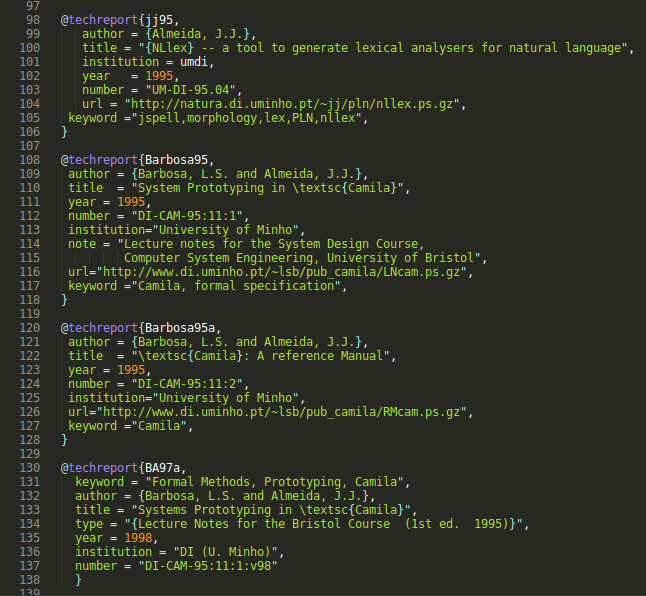
\includegraphics[scale=0.50]{Imagens/1stBib.png} \\
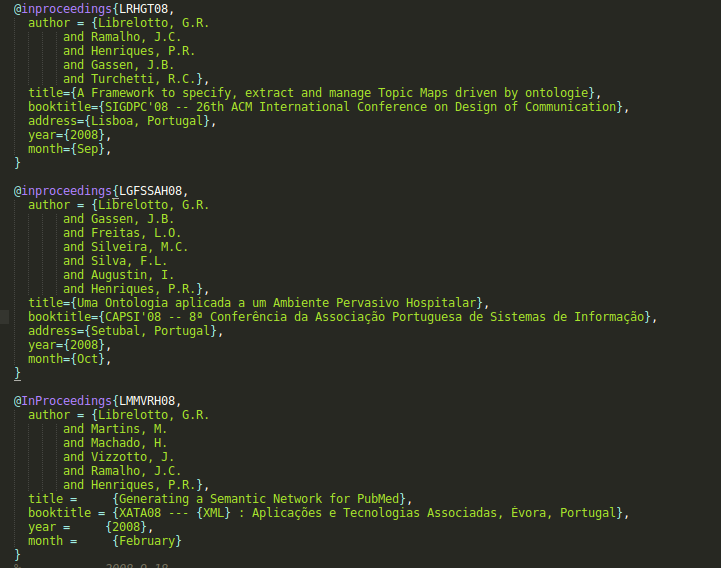
\includegraphics[scale=0.50]{Imagens/outbib1.png} \\

\subsubsection{Parte do grafo gerado}

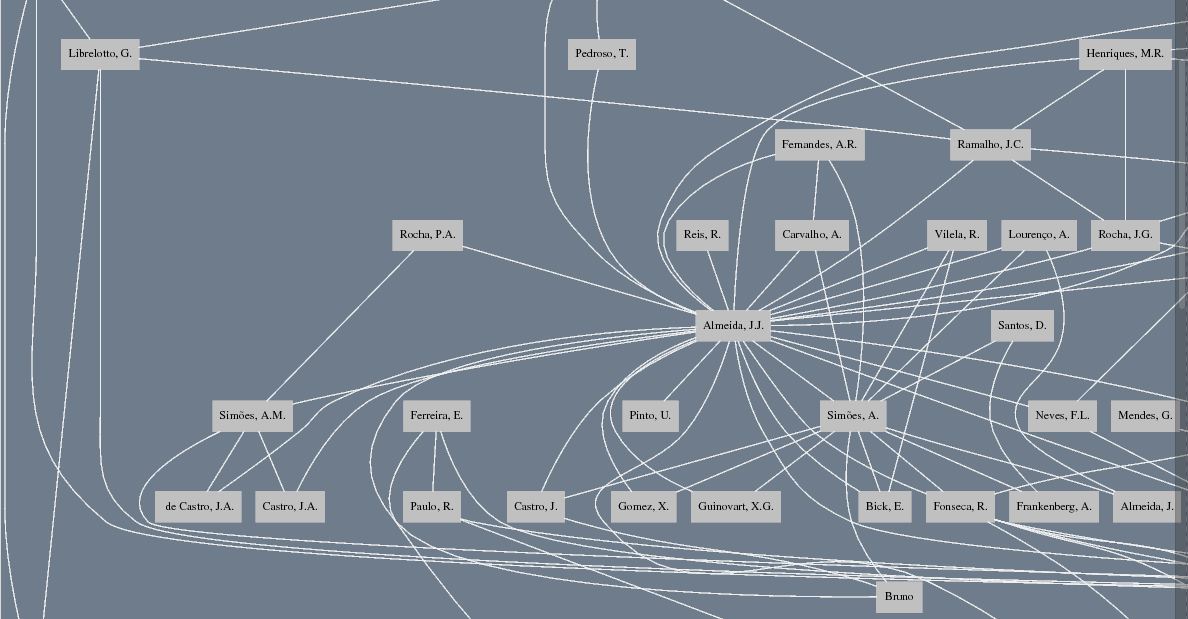
\includegraphics[scale=0.40]{Imagens/outGraph1.png} \\

\subsection{Execução para um ficheiro obtido pelo grupo de trabalho(listb.bib)}

\subsubsection{Excertos do ficheiro gerado}

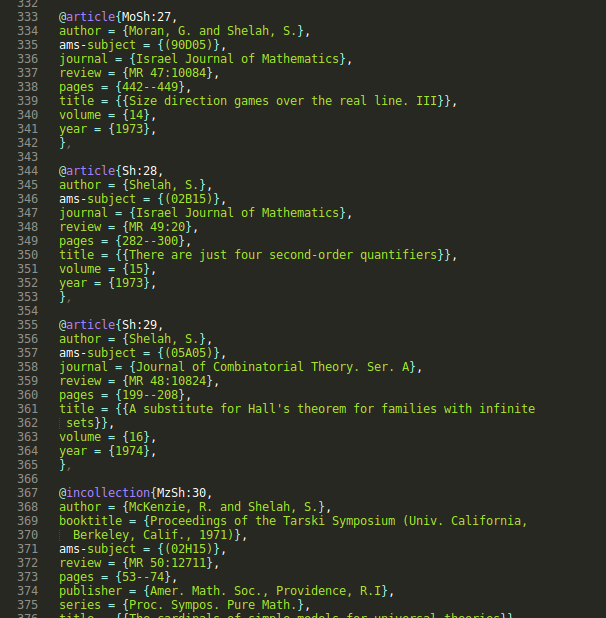
\includegraphics[scale=0.50]{Imagens/outbib2.png} \\

\subsubsection{Parte do grafo gerado}

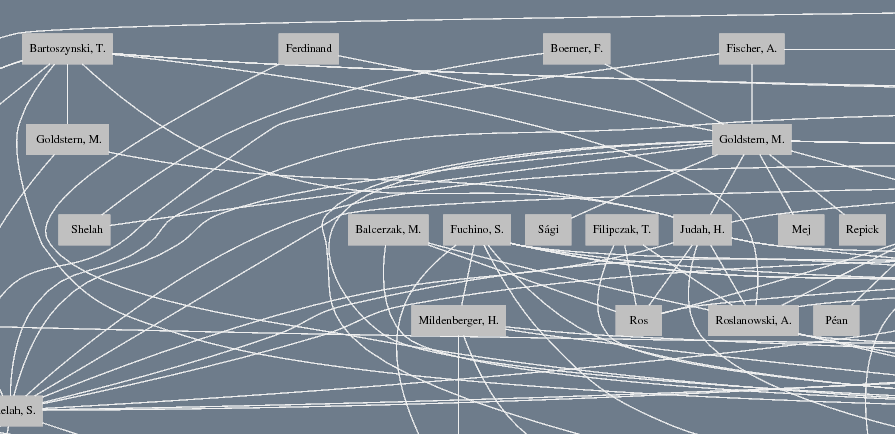
\includegraphics[scale=0.40]{Imagens/outgraph2.png}


\section{Processador de Inglês corrente}

\subsection{Alternativas, Decisões e Problemas de Implementação}
Tal como sugerido pela segunda parte do primeiro exercício prático, 
o ficheiro output deveria de estar no formato HTML. Tal e qual como 
no primeiro trabalho prático decidimos que o ficheiro deveria utilizar 
também estilos escritos em css e incluir um script(em javascript) para 
tornar possível o aparecimento de listas escondidas. 
Também foi utilizada a font-awesome para juntar icons que refletem o 
conteúdo de cada linha apresentada. O objetivo do uso destes recursos é 
tornar o conteúdo do ficheiro apelativo. Para além disso, poderíamos ter 
optado por outro tipo de estruturas de dados, como por exemplo, árvores binárias. 

No que diz respeito à implementação, achamos que a o modo de 
resolução do problema nunca poderia ser muito diferente daquele realizado. 
Seria possível acrescentar mais casos que restringissem o aparecimento de 
outras palavras que não fossem verbos. Mas, por outro lado, a adição de mais 
exceções poderia levar igualmente à supressão de verbos 
que estariam correctos a ser apresentados no ficheiro de output.

\subsection{Testes realizados e Resultados}

\subsection{Execução para ficheiro dado no enunciado(FAQ-Phyton-EN.txt)}

\subsubsection{Html obtido}
\subsubsection{Lista antes de escolher letra} 
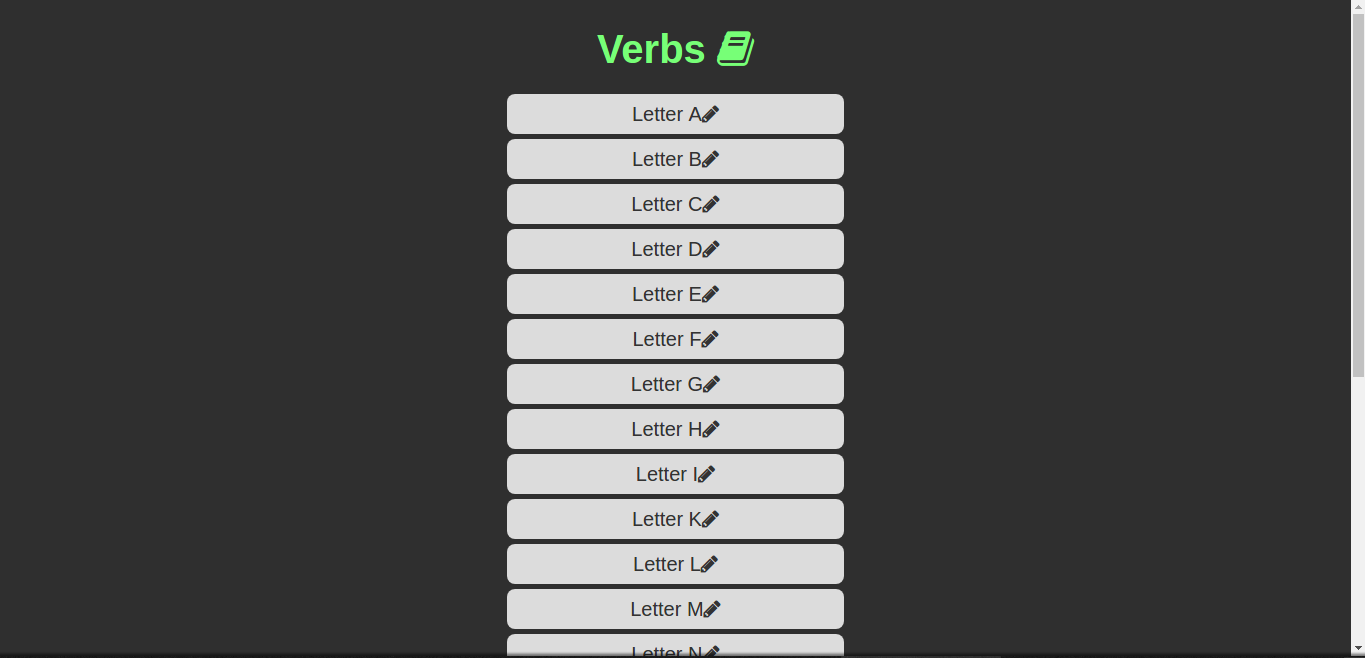
\includegraphics[scale=0.35]{Imagens/beforeClick1.png} \\
\subsubsection{Lista depois de escolher letra} 
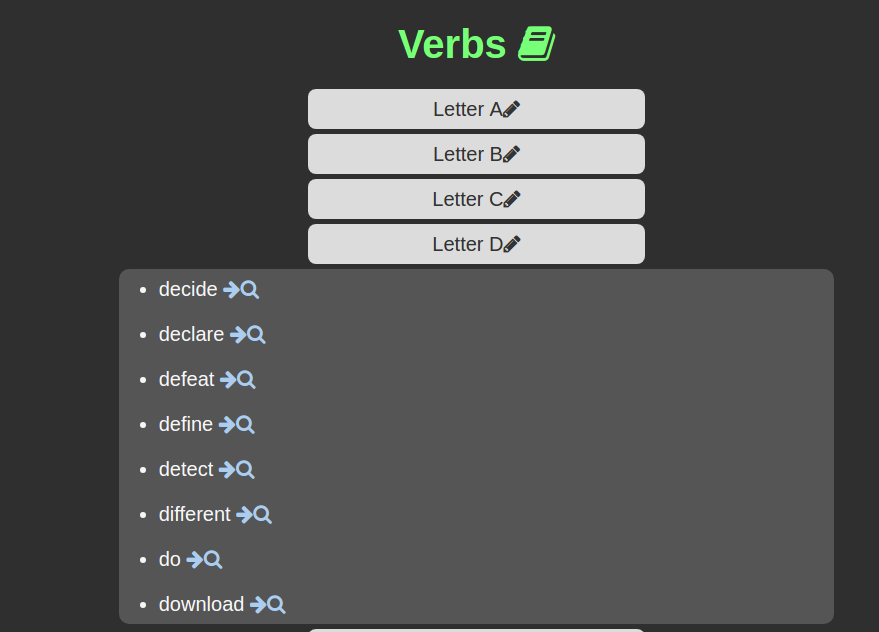
\includegraphics[scale=0.35]{Imagens/afterClick1.png} \\

\subsection{Execução para um ficheiro obtido pelo grupo(potter.txt)}

\subsubsection{Html obtido}

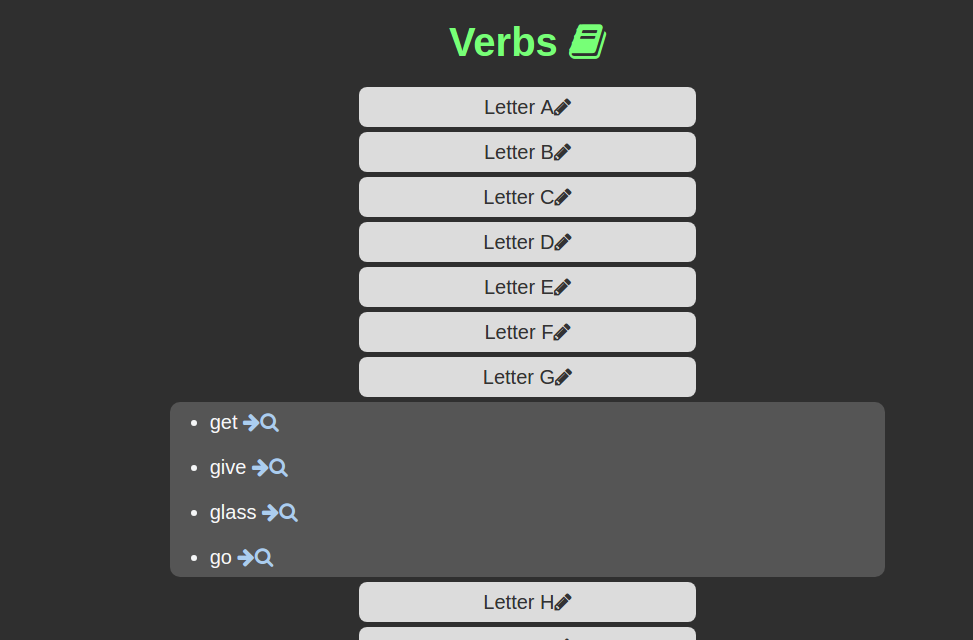
\includegraphics[scale=0.35]{Imagens/afterClick2.png}

\subsubsection{Clicando na lupa de pesquisa para get}

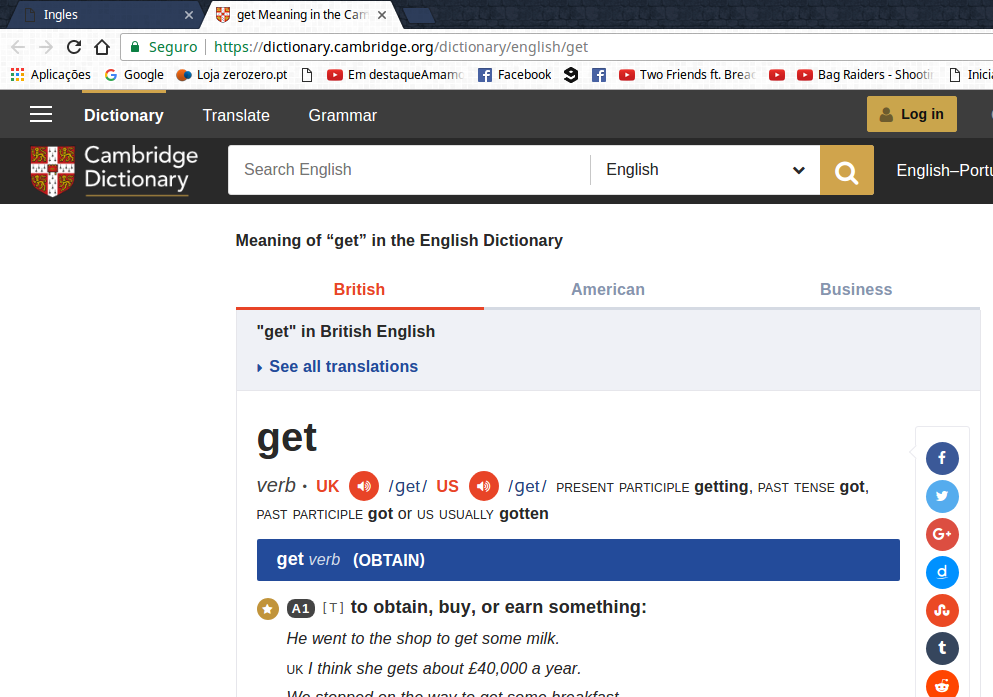
\includegraphics[scale=0.45]{Imagens/pesquisa.png}




\chapter{Conclusão} \label{concl}
Neste projeto foi possível atingir os objetivos propostos, relativos à criação de 
um Normalizador de Autores em BibTex, utilizando Expressões Regulares para a definição de padrões,
desenvolvendo Processadores de Linguagens Regulares para a filtragem e transformação de textos e 
recorrendo ao Analisador Léxico FLex para gerar filtros de texto em C.\par

Com a criação de tal Normalizador foi possível a partir de publicações, normalizar e reescrever
acentos em caracteres portuguese assim como os campos relativos aos editores e editores de modo
a serem reescritos de acordo com uma estrutura especifica. Após a normalização das publicações seria
gerado um grafo com todos os autores e ligações de colaboração entre eles, utilizando a linguagem Dotty
e processador dot para tal criação assim como o uso de expressões regulares e analisadores léxicos para
a criação do ficheiro de input do processador dot.\par

Para além da criação deste Normalizador de Autores também foi possível a realização de um Processador
de Inglês corrente, no qual seria possível a expansão de contrações da língua inglesa a partir de um dado 
texto e gerar um ficheiro html com uma lista ordenada de todos os verbos ingleses no infinitivo 
presentes no texto.\par

Com estes dois projetos foi possível estabelecer padrões de frases nos textos utilizados
através de Expressões Regulares assim como identificar as ações semânticas relativas aos padrões de frases
estabelecidos. Com o estabelecimento destes padrões foi possível a criação de um Filtro de Texto 
capaz de os reconhecer e , recorrendo ao Gerador Flex, transformar os textos de acordo com os requisitos.


\appendix
\chapter{Código do Programa para Normalizador de Autores em BibTex}

Lista-se a seguir o código  do programa  que foi desenvolvido.

\lstinputlisting{../convAcentos.fl}%input de um ficheiro
\lstinputlisting{../normNomes.fl}
\lstinputlisting{../genGraph.fl}

\chapter{Código do Programa para Processador de Inglês corrente}
\lstinputlisting{../procIngles.fl}


\bibliographystyle{alpha}
\bibliography{relprojLayout}



\end{document}

